\chapter{Sets, Functions, and Relations}
\pagebreak[4]

\section{Sets and Membership }
\subsection{}
\begin{tcolorbox}
List explicitly the elements of the set 
$$\{x:\,x<0 \text{ and } (x-1)(x+2)(x+3)=0\}$$
\end{tcolorbox}
$$\{\,-3,\, -2\}$$
$$\blacklozenge$$

\subsection{}
\begin{tcolorbox}
List the elements of the set 
$$\{x:\,3x-1  \text{ is a multiple of  } 3\}$$
\end{tcolorbox}
$$\{x:\,x= k+\frac{1}{3},\, k\in \mathbb{Z}\}$$
$$\blacklozenge$$
\subsection{}
\begin{tcolorbox}
Sketch on a number line each of the following sets.\\
(a) $\{x:\,|x-1| \leq 3  \}$\\
(b) $\{x:\,|x-1| \leq 3 \text{ and } |x| \leq 2 \}$\\
(c) $\{x:\,|x-1| \leq 3 \text{ or } |x| \leq 2 \}$
\end{tcolorbox}
\begin{figure}[H]%
    \centering
    \subfloat[]{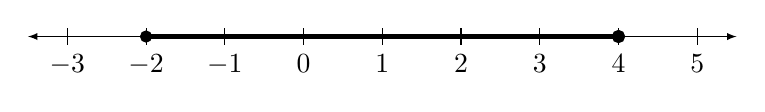
\begin{tikzpicture}
\draw[ultra thick] (-2,0) -- (4,0);
\path [draw=black, fill=black] (-2,0) circle (2pt);
\path [draw=black, fill=black, thick] (4,0.0) circle (2pt);
\draw[latex-latex, very thin] (-3.5,0) -- (5.5,0) ;
\foreach \x in  {-3,-2,-1,0,1,2,3,4,5}
\draw[shift={(\x,0)},color=black] (0pt,3pt) -- (0pt,-3pt);
\foreach \x in {-3,-2,-1,0,1,2,3,4,5}
\draw[shift={(\x,0)},color=black] (0pt,0pt) -- (0pt,-3pt) node[below] 
{$\x$};
\end{tikzpicture}}\\
    \subfloat[]{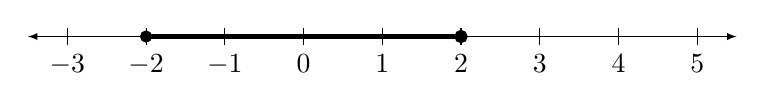
\begin{tikzpicture}
\draw[ultra thick] (-2,0) -- (2,0);
\path [draw=black, fill=black] (-2,0) circle (2pt);
\path [draw=black, fill=black, thick] (2,0.0) circle (2pt);
\draw[latex-latex, very thin] (-3.5,0) -- (5.5,0) ;
\foreach \x in  {-3,-2,-1,0,1,2,3,4,5}
\draw[shift={(\x,0)},color=black] (0pt,3pt) -- (0pt,-3pt);
\foreach \x in {-3,-2,-1,0,1,2,3,4,5}
\draw[shift={(\x,0)},color=black] (0pt,0pt) -- (0pt,-3pt) node[below] 
{$\x$};
\end{tikzpicture}}\\
    \subfloat[]{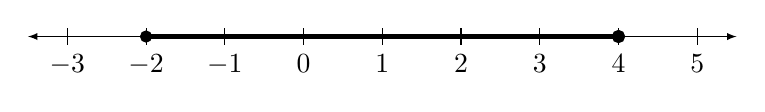
\begin{tikzpicture}
\draw[ultra thick] (-2,0) -- (4,0);
\path [draw=black, fill=black] (-2,0) circle (2pt);
\path [draw=black, fill=black, thick] (4,0.0) circle (2pt);
\draw[latex-latex, very thin] (-3.5,0) -- (5.5,0) ;
\foreach \x in  {-3,-2,-1,0,1,2,3,4,5}
\draw[shift={(\x,0)},color=black] (0pt,3pt) -- (0pt,-3pt);
\foreach \x in {-3,-2,-1,0,1,2,3,4,5}
\draw[shift={(\x,0)},color=black] (0pt,0pt) -- (0pt,-3pt) node[below] 
{$\x$};
\end{tikzpicture}}\\
%\caption{}
\label{fig:fig_p3}
\end{figure}
$$\blacklozenge$$
\newpage
\section{Some remarks on the use of the connectives \textit{and, or, implies}}
\subsection{}
\begin{tcolorbox}
Demonstrate by means of a table showing truth values that the following is a true statement for any choice of $p$ and $q$. Thus show that it is a tautology.
$$(\lnot q\Rightarrow \lnot p)\Rightarrow ( p \Rightarrow q)$$
\end{tcolorbox}
\begin{displaymath}
\begin{array}{|c c|c c|c|c|c|}
% |c c|c| means that there are three columns in the table and
% a vertical bar ’|’ will be printed on the left and right borders,
% and between the second and the third columns.
% The letter ’c’ means the value will be centered within the column,
% letter ’l’, left-aligned, and ’r’, right-aligned.
p & q &\lnot q &\lnot p &\lnot q\Rightarrow \lnot p& p\Rightarrow q&(\lnot q\Rightarrow \lnot p)\Rightarrow ( p \Rightarrow q) \\ % Use & to separate the columns
\hline % Put a horizontal line between the table header and the rest.
T & T &F&F& T&T&T\\
T & F &T&F& F&F&T\\
F & T &F&T& T&T&T\\
F & F &T&T& T&T&T\\
\end{array}
\end{displaymath}
$$\blacklozenge$$

\subsection{}
\begin{tcolorbox}
Show by means of a truth table  that the statement 
$$((p\Rightarrow q) \wedge (q\Rightarrow r))\Rightarrow (p\Rightarrow r)$$
is a tautology.
\end{tcolorbox}
\begin{displaymath}
\begin{array}{|c c c|c| c|c|c|c|}
p & q &r & p\Rightarrow q &q\Rightarrow r &(p\Rightarrow q) \wedge (q\Rightarrow r))& p\Rightarrow r&((p\Rightarrow q) \wedge (q\Rightarrow r))\Rightarrow (p\Rightarrow r)\\ % 
\hline 
T & T &T&T&T& T&T&T\\
T & T &F&T&F& F&F&T\\
T & F &T&F&T& F&T&T\\
T & F &F&F&T& F&F&T\\
F & T &T&T&T& T&T&T\\
F & T &F&T&F& F&T&T\\
F & F &T&T&T& T&T&T\\
F & F &F&T&T& T&T&T\\
\end{array}
\end{displaymath}
$$\blacklozenge$$
\subsection{}
\begin{tcolorbox}
Show by means of a truth table  that  
$$(p\wedge q) \Rightarrow (p\vee q)$$
is a tautology.
\end{tcolorbox}
\begin{displaymath}
\begin{array}{|c c|c|c|c|}
p & q &p\wedge q& p\vee q&(p\wedge q) \Rightarrow (p\vee q) \\ 
\hline 
T & T & T&T&T\\
T & F & F&F&T\\
F & T & F&T&T\\
F & F & F&F&T\\
\end{array}
\end{displaymath}
$$\blacklozenge$$
\subsection{}
\begin{tcolorbox}
Suppose that $p$ and $q$ are statements such that $(p \wedge q)$ is a false statement. Does it follow that the statement
$$(p\text{ is false}) \vee (q\text{ is false})$$is a true statement?
\end{tcolorbox}
\begin{displaymath}
\begin{array}{|c c|c|c c| c|}
p & q &p\wedge q& \lnot p&\lnot q& \lnot p \vee \lnot q\\ % Use & to separate the columns
\hline % Put a horizontal line between the table header and the rest.
T & F & F&F&T&T\\
F & T & F&T&F&T\\
F & F & F&T&T&T\\
\end{array}
\end{displaymath}
\textbf{The answer is Yes}.
$$\blacklozenge$$

\subsection{}
\begin{tcolorbox}
Negate the following statement: \textit{If two angles of a triangle have equal measure, then the length of two sides of that triangle are equal.}
\end{tcolorbox}
First we note that $\lnot(p\Rightarrow q)\Leftrightarrow (p \wedge \lnot q)$. Indeed,

\begin{displaymath}
\begin{array}{|c c|c|c | c|c| c|}

p & q &p\Rightarrow q& \lnot(p\Rightarrow q)&\lnot q&p \wedge \lnot q &\lnot(p\Rightarrow q)\Leftrightarrow (p \wedge \lnot q)\\ % Use & to separate the columns
\hline % Put a horizontal line between the table header and the rest.
T & T & T&F&F&F&T\\
T & F & F&T&T&T&T\\
F & T & T&F&F&F&T\\
F & F & T&F&T&F&T\\
\end{array}
\end{displaymath}
Putting $p$ as \textit{two angles of a triangle have equal measure} and $\lnot q$ as \textit{no two sides of that triangle have equal length} we get the true 'false' statement:\\
\textbf{Two angles of a triangle have equal measure} $\wedge$  \textbf{no two sides of that triangle have equal length}. 
$$\blacklozenge$$

\subsection{}
\begin{tcolorbox}
Write the contrapositive of the statement in Exercise 5.
\end{tcolorbox}
The contrapositive of $p\Rightarrow q$ is $\lnot q\Rightarrow \lnot p$.
Putting $\lnot p$ as \textit{no two angles of a triangle have equal measure} and $\lnot q$ as \textit{no two sides of that triangle have equal length} we get \\
\textbf{If no two sides of that triangle have equal length then no two angles of a triangle have equal measure.}
$$\blacklozenge$$

\subsection{}
\begin{tcolorbox}
Write the converse of the statement in Exercise 5.
\end{tcolorbox}
The converse of $p\Rightarrow q$ is $q\Rightarrow  p$,  giving \\
\textbf{If two sides of a triangle have equal length then  two angles of a that triangle have equal measure.}
$$\blacklozenge$$

\subsection{}
\begin{tcolorbox}
Write the contrapositive of the following statement\\
\textit{If a person belongs to Committee A, then he must be a member of Committee B and he must be a member of Committee C.}
\end{tcolorbox}
Lets put 
\begin{align*}
p\equiv \text{a person belongs to Committee A}\\
q\equiv \text{a person belongs to Committee B}\\
r\equiv \text{a person belongs to Committee C}\\
\end{align*}
then the given statement translates as 
$$p\Rightarrow (q\wedge r)$$

and the contrapositive 
$$\lnot (q\wedge r)\Rightarrow \lnot p$$
This last statement is equivalent with 
$$(\lnot q\vee \lnot r)\Rightarrow \lnot p$$ or in plain text:\\
\textbf{If a person does not belong to Committee B or C , then he is not  a member of Committee A.}
$$\blacklozenge$$

\subsection{}
\begin{tcolorbox}
Write the contrapositive of the following statement\\
$$\text{If } x\in A \text{ and } x\in B\text{, then } x \in C$$
\end{tcolorbox}
Lets put 
\begin{align*}
p\equiv x\in A\\
q\equiv x\in B\\
r\equiv x\in C\\
\end{align*}
then the given statement translates as 
$$p\wedge r\Rightarrow r$$

and the contrapositive 
$$\lnot (r)\Rightarrow \lnot (p\wedge q)$$
This last statement is equivalent with 
$$\lnot (r)\Rightarrow (\lnot p\vee \lnot q)$$ i.e:\\
$$x\notin C \Rightarrow (x\notin A \vee x\notin B)$$
$$\blacklozenge$$
\newpage
\section{Subsets}
No exercises!
\section{Union and Intersection of sets}
\subsection{}
\begin{tcolorbox}
Let $G_1$ be the graph of the equation $x^2+y^2=16$, and let $G_2$ be the graph of the equation $x^2-y^2=1$. Sketch the sets $G_1\cup G_2$ and $G_1\cap G_2$.
\end{tcolorbox}
\begin{figure}[H]%
    \centering
\begin{tikzpicture}
\begin{axis}[ 
xlabel=$x$,
ylabel=$y$,
axis x line=center, xlabel style={anchor=north west},
axis y line=center, ylabel style={anchor=south west},
xmin=-4.5,
xmax=4.5,
ymin=-5.5,
ymax=5.5,
axis line style={thick, shorten > = -0.5cm, shorten < = -0.5cm},
samples=50,
unit vector ratio*=1 1,
]

\addplot [domain=-4:4, thick, black, smooth]{sqrt(16-x^2)};
\addplot [domain=-4:4, thick, black, smooth]{-sqrt(16-x^2)};
\addplot [domain=-4:-1, thick, black, smooth,<-,>=latex]{sqrt(x^2-1)};
\addplot [domain=-4:-1, thick, black, smooth,,<-,>=latex]{-sqrt(x^2-1)};    
\addplot [domain=1:4, thick, black, smooth,->,>=latex]{sqrt(x^2-1)};
\addplot [domain=1:4, thick, black, smooth,->,>=latex]{-sqrt(x^2-1)};
\coordinate (A) at (axis cs:2.91547,2.7386) {};
\coordinate (B) at (axis cs:+2.91547,-2.7386) {};
\coordinate (C) at (axis cs:-2.91547,2.7386) {};
\coordinate (D) at (axis cs:-2.91547,-2.7386) {};
\draw [fill=white] (A) circle [radius=10.05];
\draw [fill= white] (B) circle [radius=10.05];
\draw [fill= white] (C) circle [radius=10.05];
\draw [fill= white] (D) circle [radius=10.05];
\node[anchor=south ] at (A) {A};
\node[anchor=north ] at (B) {B};
\node[anchor=south ] at (C) {D};
\node[anchor=north ] at (D) {C};

\end{axis};
\coordinate (S) at (3,5.5) {};
\node[anchor=north west] at (S) {$G_1\cap G_2\equiv \{A,B,C,D\}$};
%\path (current axis.south west) +(-0.5cm,-0.5cm) (current axis.north east) +(0.5cm,0.5cm);


\end{tikzpicture}\\
%\caption{}
\label{fig:fig_p8a}
\end{figure}
$G_1\cup G_2$ contains all the points defined by the graphs $G_1$ and $G_2$. 
$G_1\cap G_2\equiv \{A,B,C,D\}$ contains the 4 points at the intersection of the two graphs.
$$\blacklozenge$$
\newpage
\subsection{}
\begin{tcolorbox}
We define the sets $A,\, B,\,C$ as follows: $A=\{(x,y):x^2+y^2\le 9\}$, $ B=\{(x,y):x+y\ge 3\}$, $C=\{(x,y):x\ge 0\}$.\\Draw sketches of each of the following sets:
\begin{align*}
\begin{array}{ll}
(a)&A\cup (B\cup C)\\
(b)&A\cap (B\cup C)\\
(c)&(A\cap B)\cup (A\cap C)\\
(d)&(A\cup B)\cup C\\
(e)&A\cup (B\cap C)\\
(f)&(A\cup B)\cap (A\cup C)\\
\end{array}
\end{align*}
\end{tcolorbox}
\begin{figure}[H]%
    \centering
    \begin{tikzpicture}
\begin{axis}[ 
xlabel=$x$,
ylabel=$y$,
axis x line=center, xlabel style={anchor=north west},
axis y line=center, ylabel style={anchor=south west},
xmin=-4.5,
xmax=5.9,
ymin=-5.5,
ymax=5.5,
axis line style={thick, shorten > = -0.5cm, shorten < = -0.5cm},
samples=50,
unit vector ratio*=1 1,
]

\addplot [domain=-3:3, thick, black, smooth,pattern={Lines[
                  distance=2mm,
                  angle=-45
                 ]},
        pattern color=gray!50]{sqrt(9-x^2)};
\addplot [domain=-3:3, thick, black, smooth,pattern={Lines[
                  distance=2mm,
                  angle=-45
                 ]},
        pattern color=gray!50]{-sqrt(9-x^2)};
\addplot [domain=-5:5, thick, black, smooth,<-,>=latex]{3-x};

\coordinate (A) at (axis cs:5,-2) {};
\coordinate (B) at (axis cs:-4,7) {};
\coordinate (C) at (axis cs:-4,9) {};
\coordinate (D) at (axis cs:5,9) {};
\path[ pattern={Lines[
                  distance=2mm,
                  angle=45
                 ]},
        pattern color=gray!50](A)--(B)--(C)--(D);
\path[ pattern={Lines[
                  distance=2mm,
                  angle=0
                 ]},
        pattern color=gray!50] (axis cs:0,-6) --(axis cs:3,-6)--(axis cs:3,6)--(axis cs:0,6)--(axis cs:0,6);
%\node[anchor=south ] at (A) {A};
\begin{scope}
\coordinate (S) at (axis cs:-1.5,1.5) {};
\coordinate (St) at (axis cs:-3.3,3.5) {};
\draw [fill= white] (S) circle [radius=10.05];
\node[above] at (St) {$A$};
\draw[-{Latex[length=2mm]}] (St) .. controls ([xshift=-1cm] S) and ( S) .. (S);

\coordinate (P) at (axis cs:2,-4) {};
\coordinate (Pt) at (axis cs:4,-3.5) {};
\draw [fill= white] (P) circle [radius=10.05];
\node[above] at (Pt) {$C$};
\draw[-{Latex[length=2mm]}] (Pt) .. controls ([xshift=-0.5cm] Pt) and ( P) .. (P);


\coordinate (T) at (axis cs:4,1.5) {};
\coordinate (Tt) at (axis cs:5.5,3.5) {};
\draw [fill= white] (T) circle [radius=10.05];
\node[above] at (Tt) {$B$};
\draw[-{Latex[length=2mm]}] (Tt) .. controls ([xshift=1cm] T) and ( T) .. (T);

\end{scope}
\end{axis};
\end{tikzpicture}
\caption{The 3 sets $A,\,B,\, C$}
\label{fig:fig_p8b}
\end{figure}
\begin{figure}[H]%
    \centering
    \subfloat[$A\cup (B\cup C)$ ]{\begin{tikzpicture}
\begin{axis}[ 
xlabel=$x$,
ylabel=$y$,
axis x line=center, xlabel style={anchor=north west},
axis y line=center, ylabel style={anchor=south west},
xmin=-4.5,
xmax=5.9,
ymin=-5.5,
ymax=5.5,
axis line style={thick, shorten > = -0.5cm, shorten < = -0.5cm},
samples=50,
unit vector ratio*=1 1,
]

\addplot [domain=-3:3, thick, black, smooth,pattern={Lines[
                  distance=2mm,
                  angle=45
                 ]},
        pattern color=gray!50]{sqrt(9-x^2)};
\addplot [domain=-3:3, thick, black, smooth,pattern={Lines[
                  distance=2mm,
                  angle=45
                 ]},
        pattern color=gray!50]{-sqrt(9-x^2)};
\addplot [domain=-5:5, thick, black, smooth,<-,>=latex]{3-x};

\coordinate (A) at (axis cs:5,-2) {};
\coordinate (B) at (axis cs:-4,7) {};
\coordinate (C) at (axis cs:-4,9) {};
\coordinate (D) at (axis cs:5,9) {};
\path[ pattern={Lines[
                  distance=2mm,
                  angle=45
                 ]},
        pattern color=gray!50](A)--(B)--(C)--(D);
\path[ pattern={Lines[
                  distance=2mm,
                  angle=45
                 ]},
        pattern color=gray!50] (axis cs:0,-6) --(axis cs:6,-6)--(axis cs:6,6)--(axis cs:0,6)--(axis cs:0,6);

\end{axis};
\end{tikzpicture}}
    \subfloat[$A\cap (B\cup C)$]{\begin{tikzpicture}
\begin{axis}[
xlabel=$x$,
ylabel=$y$,
axis x line=center, xlabel style={anchor=north west},
axis y line=center, ylabel style={anchor=south west},
xmin=-4.5,
xmax=5.9,
ymin=-5.5,
ymax=5.5,
axis line style={thick, shorten > = -0.5cm, shorten < = -0.5cm},
samples=50,
unit vector ratio*=1 1,
]

\addplot [domain=-3:3, thick, black, smooth]{sqrt(9-x^2)};
\addplot [domain=-3:3, thick, black, smooth]{-sqrt(9-x^2)};
\addplot [domain=0:3, thick, black, smooth,pattern={Lines[
                  distance=2mm,
                  angle=45
                 ]},
        pattern color=gray!50]{sqrt(9-x^2)};
\addplot [domain=-0:3, thick, black, smooth,pattern={Lines[
                  distance=2mm,
                  angle=45
                 ]},
        pattern color=gray!50]{-sqrt(9-x^2)};
\addplot [domain=-5:5, thick, black, smooth]{3-x};
% Draw semicircle
\fill[pattern={Lines[
                  distance=2mm,
                  angle=45
                 ]},
        pattern color=gray!50]  (axis cs:3,0) arc (0:-90:300) |- cycle;
\fill[pattern={Lines[
                  distance=2mm,
                  angle=45
                 ]},
        pattern color=gray!50]  (axis cs:3,0) arc (0:90:300) |- cycle;
\end{axis};
\end{tikzpicture}}\\
    \subfloat[$(A\cap B)\cup (A\cap C)$]{\begin{tikzpicture}
\begin{axis}[
xlabel=$x$,
ylabel=$y$,
axis x line=center, xlabel style={anchor=north west},
axis y line=center, ylabel style={anchor=south west},
xmin=-4.5,
xmax=5.9,
ymin=-5.5,
ymax=5.5,
axis line style={thick, shorten > = -0.5cm, shorten < = -0.5cm},
samples=50,
unit vector ratio*=1 1,
]

\addplot [domain=-3:3, thick, black, smooth]{sqrt(9-x^2)};
\addplot [domain=-3:3, thick, black, smooth]{-sqrt(9-x^2)};
\addplot [domain=0:3, thick, black, smooth,pattern={Lines[
                  distance=2mm,
                  angle=45
                 ]},
        pattern color=gray!50]{sqrt(9-x^2)};
\addplot [domain=-0:3, thick, black, smooth,pattern={Lines[
                  distance=2mm,
                  angle=45
                 ]},
        pattern color=gray!50]{-sqrt(9-x^2)};
\addplot [domain=-5:5, thick, black, smooth]{3-x};
% Draw semicircle
\fill[pattern={Lines[
                  distance=2mm,
                  angle=45
                 ]},
        pattern color=gray!50]  (axis cs:3,0) arc (0:-90:300) |- cycle;
\fill[pattern={Lines[
                  distance=2mm,
                  angle=45
                 ]},
        pattern color=gray!50]  (axis cs:3,0) arc (0:90:300) |- cycle;
\end{axis};
\end{tikzpicture}}
    \subfloat[$(A\cup B)\cup C$]{\begin{tikzpicture}
\begin{axis}[ 
xlabel=$x$,
ylabel=$y$,
axis x line=center, xlabel style={anchor=north west},
axis y line=center, ylabel style={anchor=south west},
xmin=-4.5,
xmax=5.9,
ymin=-5.5,
ymax=5.5,
axis line style={thick, shorten > = -0.5cm, shorten < = -0.5cm},
samples=50,
unit vector ratio*=1 1,
]

\addplot [domain=-3:3, thick, black, smooth,pattern={Lines[
                  distance=2mm,
                  angle=45
                 ]},
        pattern color=gray!50]{sqrt(9-x^2)};
\addplot [domain=-3:3, thick, black, smooth,pattern={Lines[
                  distance=2mm,
                  angle=45
                 ]},
        pattern color=gray!50]{-sqrt(9-x^2)};
\addplot [domain=-5:5, thick, black, smooth,<-,>=latex]{3-x};

\coordinate (A) at (axis cs:5,-2) {};
\coordinate (B) at (axis cs:-4,7) {};
\coordinate (C) at (axis cs:-4,9) {};
\coordinate (D) at (axis cs:5,9) {};
\path[ pattern={Lines[
                  distance=2mm,
                  angle=45
                 ]},
        pattern color=gray!50](A)--(B)--(C)--(D);
\path[ pattern={Lines[
                  distance=2mm,
                  angle=45
                 ]},
        pattern color=gray!50] (axis cs:0,-6) --(axis cs:6,-6)--(axis cs:6,6)--(axis cs:0,6)--(axis cs:0,6);

\end{axis};
\end{tikzpicture}}\\
    \subfloat[$A\cup (B\cap C)$]{\begin{tikzpicture}
\begin{axis}[
xlabel=$x$,
ylabel=$y$,
axis x line=center, xlabel style={anchor=north west},
axis y line=center, ylabel style={anchor=south west},
xmin=-4.5,
xmax=5.9,
ymin=-5.5,
ymax=5.5,
axis line style={thick, shorten > = -0.5cm, shorten < = -0.5cm},
samples=50,
unit vector ratio*=1 1,
]

\addplot [domain=-3:3, thick, black, smooth,,pattern={Lines[
                  distance=2mm,
                  angle=45
                 ]},
        pattern color=gray!50]{sqrt(9-x^2)};
\addplot [domain=-3:3, thick, black, smooth,,pattern={Lines[
                  distance=2mm,
                  angle=45
                 ]},
        pattern color=gray!50]{-sqrt(9-x^2)};
\addplot [domain=0:3, thick, black, smooth,pattern={Lines[
                  distance=2mm,
                  angle=45
                 ]},
        pattern color=gray!50]{sqrt(9-x^2)};
\addplot [domain=-0:3, thick, black, smooth,pattern={Lines[
                  distance=2mm,
                  angle=45
                 ]},
        pattern color=gray!50]{-sqrt(9-x^2)};
\addplot [domain=-5:5, thick, black, smooth]{3-x};
% Draw semicircle
\fill[pattern={Lines[
                  distance=2mm,
                  angle=45
                 ]},
        pattern color=gray!50]  (axis cs:3,0) arc (0:-90:300) |- cycle;
\fill[pattern={Lines[
                  distance=2mm,
                  angle=45
                 ]},
        pattern color=gray!50]  (axis cs:0,3)--(axis cs:5,-2)--(axis cs:5,6)--(axis cs:0,6);
\end{axis};
\end{tikzpicture}}
    \subfloat[$(A\cup B)\cap (A\cup C)$]{\begin{tikzpicture}
\begin{axis}[
xlabel=$x$,
ylabel=$y$,
axis x line=center, xlabel style={anchor=north west},
axis y line=center, ylabel style={anchor=south west},
xmin=-4.5,
xmax=5.9,
ymin=-5.5,
ymax=5.5,
axis line style={thick, shorten > = -0.5cm, shorten < = -0.5cm},
samples=50,
unit vector ratio*=1 1,
]

\addplot [domain=-3:3, thick, black, smooth,,pattern={Lines[
                  distance=2mm,
                  angle=45
                 ]},
        pattern color=gray!50]{sqrt(9-x^2)};
\addplot [domain=-3:3, thick, black, smooth,,pattern={Lines[
                  distance=2mm,
                  angle=45
                 ]},
        pattern color=gray!50]{-sqrt(9-x^2)};
\addplot [domain=0:3, thick, black, smooth,pattern={Lines[
                  distance=2mm,
                  angle=45
                 ]},
        pattern color=gray!50]{sqrt(9-x^2)};
\addplot [domain=-0:3, thick, black, smooth,pattern={Lines[
                  distance=2mm,
                  angle=45
                 ]},
        pattern color=gray!50]{-sqrt(9-x^2)};
\addplot [domain=-5:5, thick, black, smooth]{3-x};
% Draw semicircle
\fill[pattern={Lines[
                  distance=2mm,
                  angle=45
                 ]},
        pattern color=gray!50]  (axis cs:3,0) arc (0:-90:300) |- cycle;
\fill[pattern={Lines[
                  distance=2mm,
                  angle=45
                 ]},
        pattern color=gray!50]  (axis cs:0,3)--(axis cs:5,-2)--(axis cs:5,6)--(axis cs:0,6);
\end{axis};
\end{tikzpicture}}\\
%\caption{}
\label{fig:fig_p8b}
\end{figure}
$$\blacklozenge$$